\chapter{Implementation}

\section{Components}

\subsection{User Interface}
\begin{figure}
	\centering
	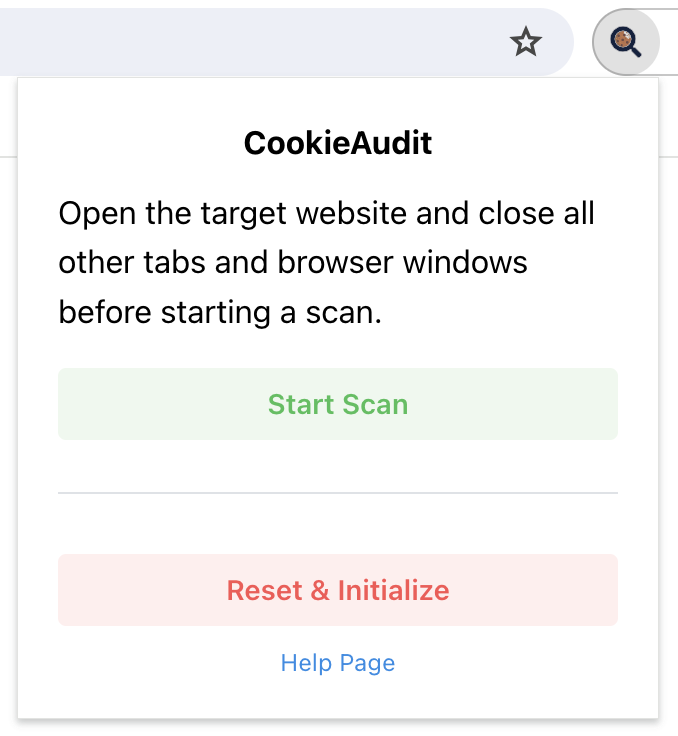
\includegraphics[width=0.5\linewidth]{screenshot_popup.png}
	\caption{Popup window of CookieAudit}
	\label{fig:screenshot-popup}
\end{figure}
The main way for a user to interact with a browser extension is via the Popup.
It is a small window which can be opened by clicking the extension's action icon.
It is programmed using the same technologies as websites: HTML, CSS and JavaScript.
In CookieAudit, the user can start a scan of a website, stop it, or download the report summarizing the scan results via the Popup.
Furthermore, CookieAudit displays current information about the progress of the scan inside the Popup.
For the development of the Popup user interface we decided to use the JavaScript library React.
React provides a declarative programming model that keeps the displayed data in sync with the underlying data storage.

\subsection{Cookie Notice Selection}
CookieAudit aims to analyze and interact with arbitrary cookie notices automatically.
Unfortunately, cookie notices are just regular HTML elements.
Next, we will give an overview of the possible heuristics based approaches to identify cookie notices.
\subsubsection{Automated Notice Selection}
\paragraph{Crowd-sourced Selectors}
HTML elements can be identified with \emph{selectors}. 
Crowd sourced efforts, such as EasyList Cookie (\href{https://github.com/easylist/easylist}{github.com/easylist/easylist}), maintain lists of cookie notice selectors.
Automated crawlers by Kampanos et al.~\cite{kampanos2021accept} and Bouhoula et al.~\cite{bouhoula2023automated} have used EasyList to find potential cookie notices on websites .
\paragraph{Stack Level}
The \emph{z-index} is a CSS property of HTML elements that makes elements with a high index appear above elements with a low index. 
Because a user should quickly see a cookie notice, websites can use a high \emph{z-index} on the notice to let it cover the rest of the website. 
This qualifier has been used by Khandelwal et al.~\cite{khandelwal2023automated} and Bouhoula et al.~\cite{bouhoula2023automated}.

\subsubsection{User Aided Selection}
Fortunately, CookieAudit is a browser extension that is used manually.
We can therefore rely on user help by using a cookie notice selector tool.
To identify a notice, the user only needs to hover over the correct element and then confirm his selection.

\subsection{Dark Pattern Detection}
\subsection{Managing Page Loads and Changes}
\subsection{Report Creation}
